\documentclass{beamer}

\usepackage{xcolor}
\usepackage{lmodern}
\usepackage{geometry}
\usepackage{calc}
\usepackage{textpos}
\usepackage{ragged2e}
\usepackage{hyperref}

\usepackage{cite}
\usepackage{amsmath}
\usepackage{xspace}
\usepackage{graphicx}
\usepackage{svg}
\usepackage{cleveref}
\usepackage{framed}
\usepackage{comment}
\usepackage{float}
\usepackage{rotating}
\usepackage{xstring}

%\usepackage{graphicx}
%\usepackage{mathtools}
%\usepackage{framed}
%\usepackage{cleveref}
%\usepackage{hyperref}
\usepackage[]{algorithm2e}
%\usepackage{subcaption}

\geometry{paperwidth=36in,paperheight=24in,hmargin=2cm}
\usetheme{poster}
\usecolortheme{poster}

\newcommand{\SHR}{Shrinkwrap\xspace}

\newenvironment{BlueBlock}[1]
{\begin{alertblock}{#1\rule{0pt}{2.3ex}} \vspace*{16pt}}
{\end{alertblock}}

\newenvironment{GoldBlock}[1]
{\begin{exampleblock}{#1\rule{0pt}{2.3ex}} \vspace*{16pt}}
{\end{exampleblock}}

\begin{document}
\begin{frame}[fragile]
\frametitle{
  {\fontsize{55pt}{55pt}\selectfont
  \textbf{Deploying Complex Software Stacks in Containers at HPC Sites}} \\ \vspace{32pt}
  {\fontsize{48pt}{48pt}\selectfont
  Tim Shaffer, Nicholas Hazekamp, and Douglas Thain}
}

\begin{minipage}[t][0.93\textheight]{0.32\textwidth}

\begin{BlueBlock}{Abstract}
\parbox{\linewidth}{
Scientific applications often depend on large,
complex software repositories containing libraries, tools,
and frameworks in multiple versions and platforms to support many researchers.
Such repositories are distributed to hundreds of major computing facilities around the world using a global filesystem like CVMFS.
However, not all HPC facilities permit execution nodes to mount and access global network resources,
instead requiring applications to make use of local filesystems or container technologies.
In this work, we present a technique for efficiently \emph{projecting} global filesystems into local resources.
This consists of creating minimal local containers that meet the needs of specific jobs,
and balancing between the extremes of having many small single-purpose containers and having large all-purpose containers.
We also simulate container management of production HEP workloads and illustrate how researchers can balance the storage and compute capabilities of their execution sites to achieve more than twofold decrease in data duplication across container images.
}
\end{BlueBlock}

\vfill

\begin{BlueBlock}{Global file system access methods}
\parbox{0.6\linewidth}{
\fbox{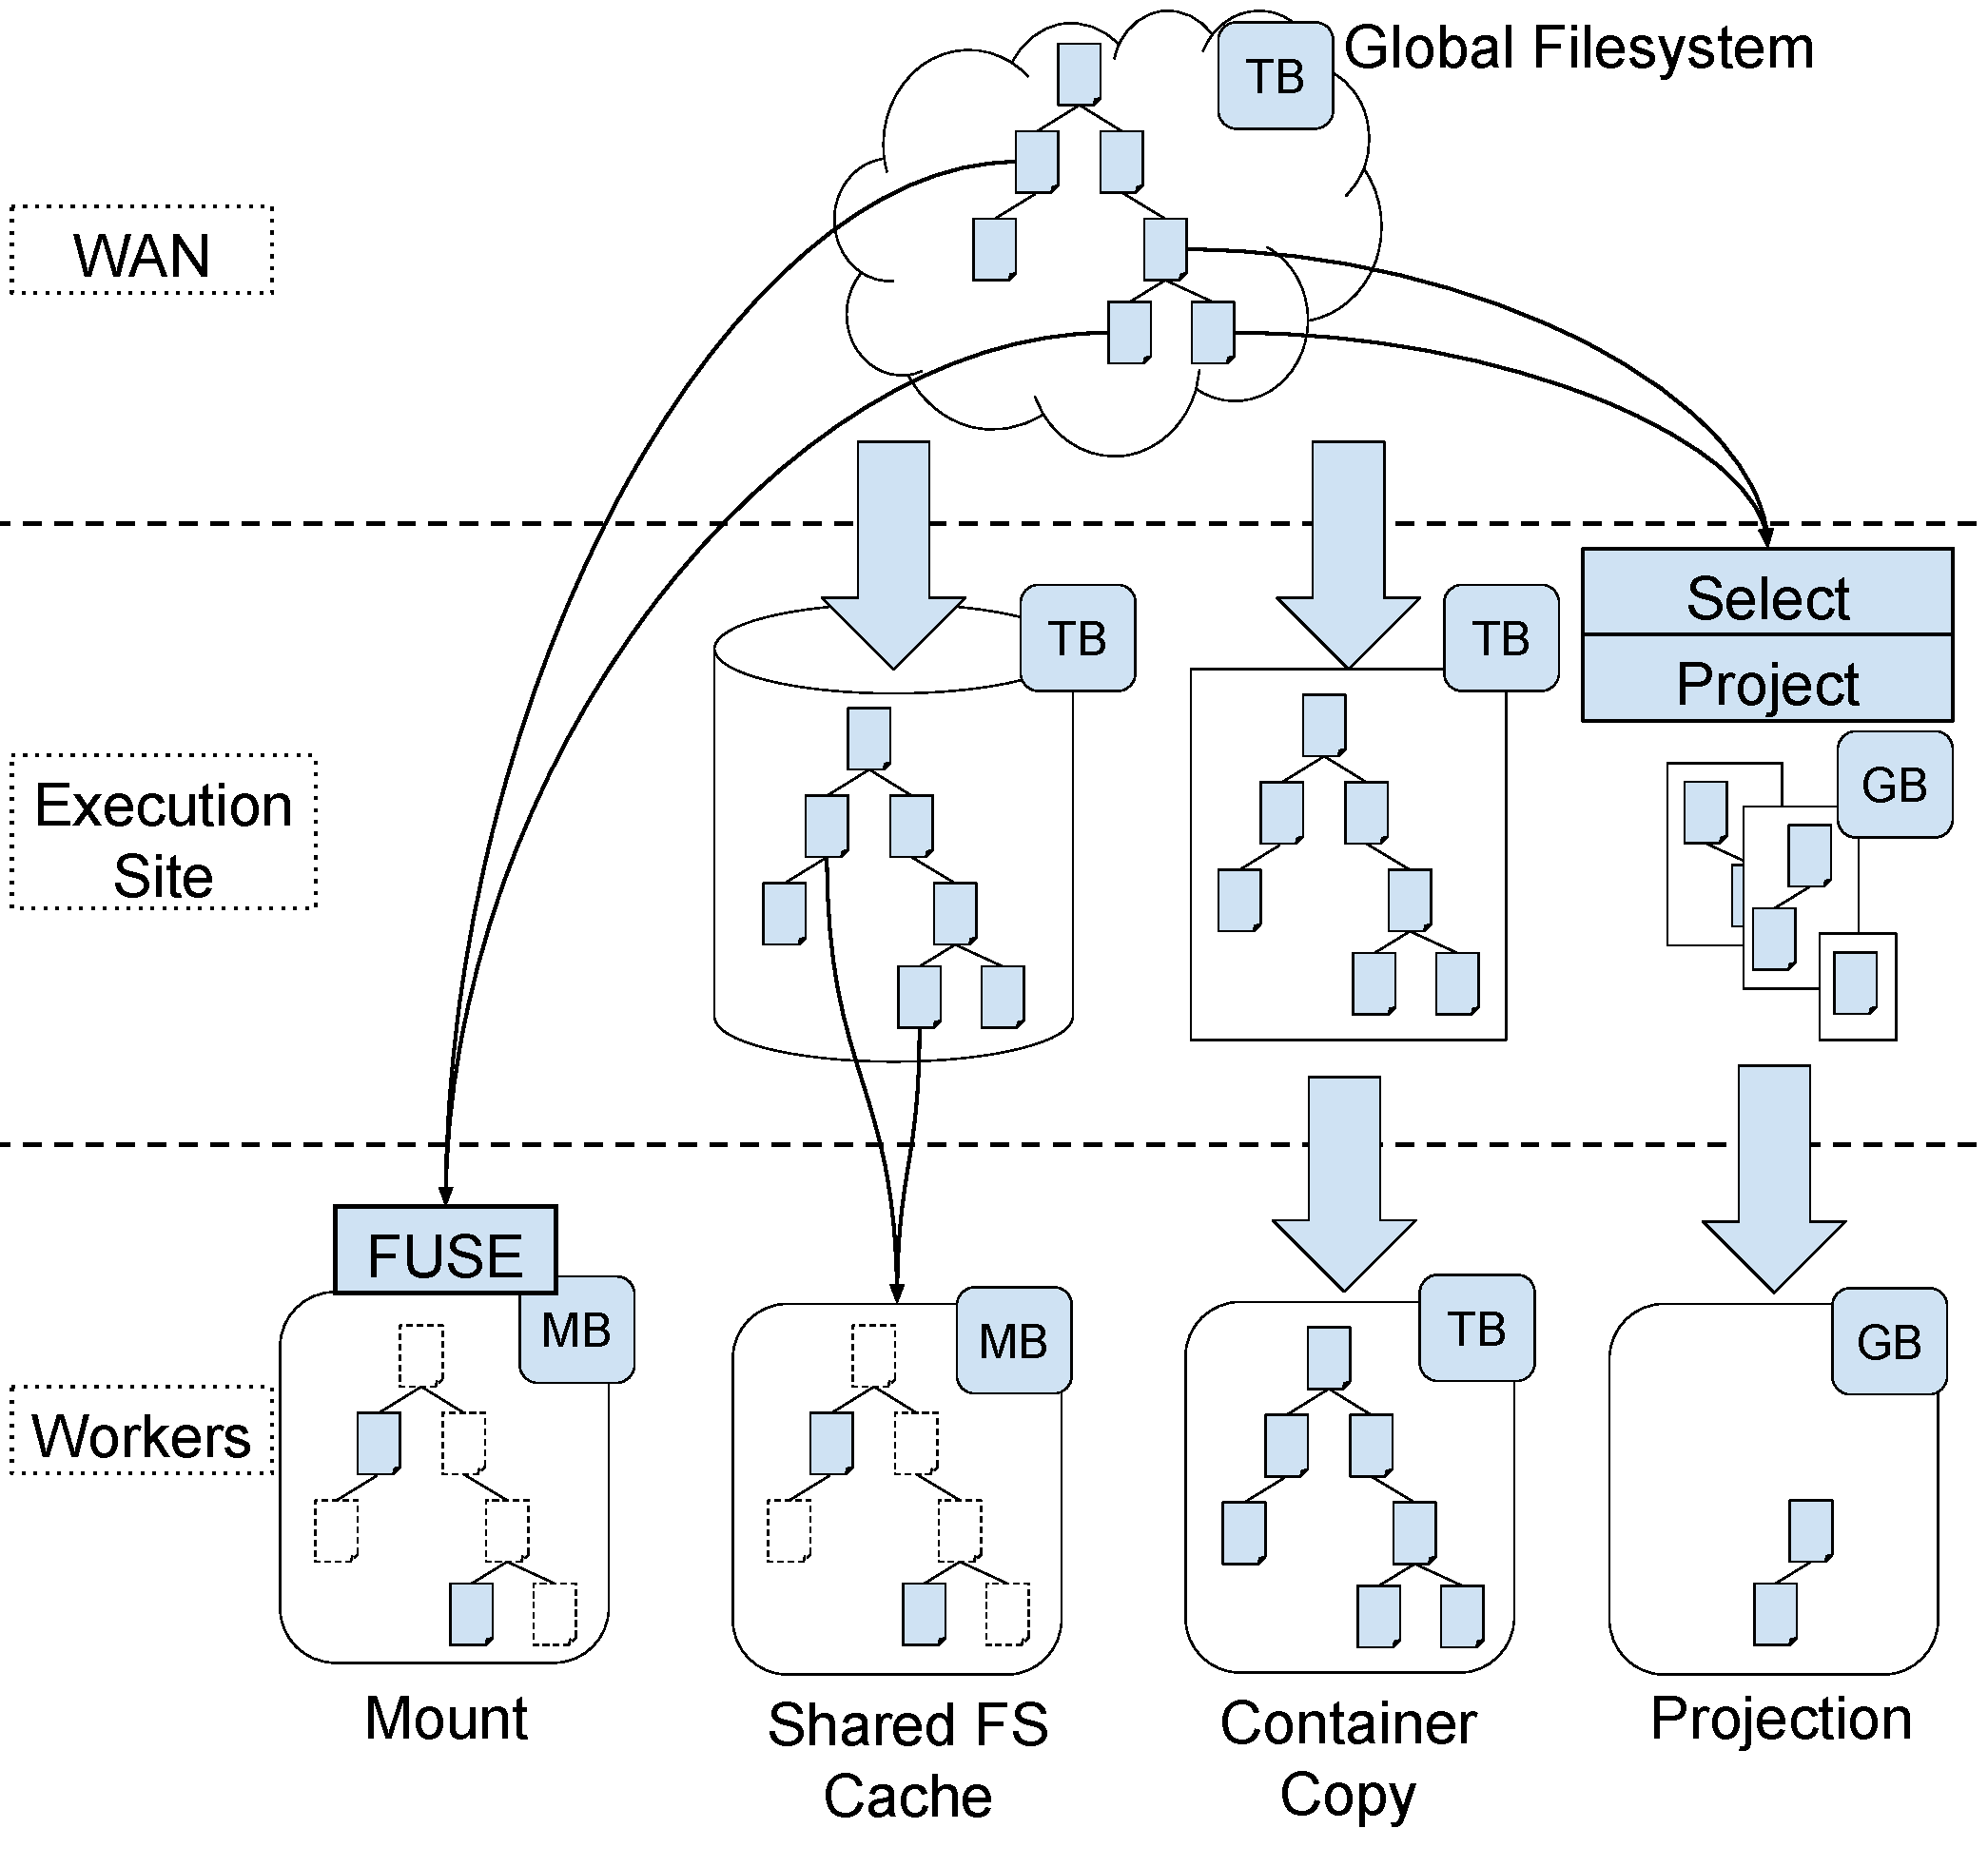
\includegraphics[width=\linewidth]{drawings/methods.pdf}}
}
\hfill
\parbox{0.35\linewidth}{
\vspace*{1.5ex}

\textbf{Mounting.}  Simplest approach,
but often not possible at HPC sites
for security, efficiency, or configuration reasons.

\textbf{Shared FS Cache.}
Copy the entire repo to a
shared FS at the site;
generally
not efficient for delivering software collections (deep directories, many small files).
}

\vspace*{0.5ex}

\parbox{\linewidth}{
\textbf{Container Copy.}
Deploy complex software tree into a container,
so the underlying filesystem delivers a single large image file to worker nodes.
Entire repo (measured in TB) is likely to exceed practical limits on container size.

\textbf{Projection.}
Only project the
required subset of the global repo into a container.
Reasonable size to efficiently transfer to each worker node,
but each job may need a different container image.
}
\end{BlueBlock}

\end{minipage}\hfill
\begin{minipage}[t][0.93\textheight]{0.32\textwidth}

\begin{BlueBlock}{CVMFS}
\parbox{\linewidth}{
The CernVM File System (CVMFS) filesystem is used as the primary means to publish the software used by all of the major LHC
experiments to hundreds of computing sites around the world on the Worldwide LHC Computing Grid (WLCG).
Each WLCG site provides computational resources for analyzing particle collision events and running simulations.
Worker nodes at each site must be configured to mount CVMFS as a prerequisite to performing any computational tasks.

%\vspace*{1ex}
\begin{center}
\begin{tabular}{l|r r r r}
& Inode & Apparent & Deduped \\
& Count & Size & Size \\ \hline
ATLAS Container \rule{0pt}{2.3ex} & 1.25 M & 84.8 GB & 59.4 GB \\
ATLAS Full Repo & 124 M & 6.42 TB & 2.61 TB  \\
CMS Container & 6.77 K & 592 MB & 592 MB  \\
CMS Full Repo & 144 M & 7.71 TB & 5.79 TB  \\
\end{tabular}
\end{center}
%\vspace*{1ex}

With the rapidly increasing demands of the LHC experiments at CERN,
use of national-scale HPC resources such as NERSC facilities in the United States and Piz Daint at the Swiss CSCS HPC center could be key in meeting the computational demands following the LHC's high-luminosity upgrade.
Unfortunately, HPC sites are less able to cater to the requirements of CVMFS.
}
\end{BlueBlock}

\vfill

\begin{BlueBlock}{Shrinkwrap}
\centering
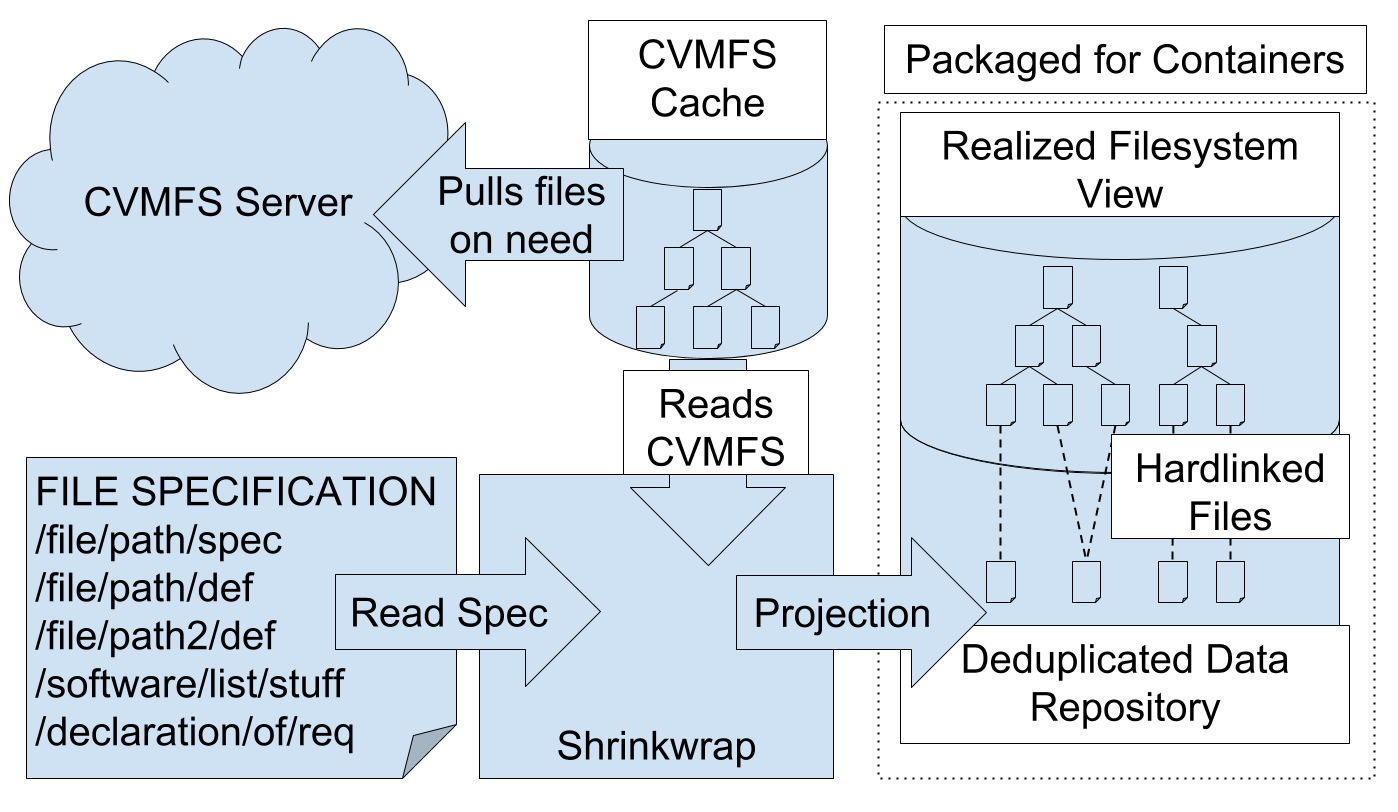
\includegraphics[width=0.8\linewidth]{drawings/shrinkwrap-structure.png}

\parbox{\linewidth}{
We created the \SHR utility to
create efficient and lightweight projections of CVMFS repositories
based on user specifications.
\SHR exploits the design of CVMFS to deduplicate
data and capture specific repository versions offered by CVMFS.
\SHR uses the CVMFS client library
to allow user-level access,
without requiring administrative privileges.
}
\end{BlueBlock}


\end{minipage}\hfill
\begin{minipage}[t][0.93\textheight]{0.32\textwidth}

\begin{BlueBlock}{Online Storage Optimization}
\parbox{\linewidth}{
Rather than relying on administrators or end users to manually manage a large number of images,
we want an online method to to efficiently satisfy the dependency requirements for submitted jobs.
The fundamental operation for our storage optimization strategy will be merging container specifications that are ``close enough''.
We use the Jaccard distance,
\[
d_j(A, B) = 1 - \frac{|A \cap B|}{|A \cup B|} = \frac{|A \cup B| - |A \cap B|}{|A \cup B|}
\]
to quickly identify cached projections that are similar.
We define $\alpha$ as the ``globbiness'' of the system.
Small choice of $\alpha$ requires that projections be extremely close before considering them for merging.
Larger $\alpha$ makes it more likely for images to be considered similar and merged
to serve multiple tasks.
}
\end{BlueBlock}

\vfill

\begin{BlueBlock}{Limits on efficiency}
\centering

\parbox{\linewidth}{
We simulated HEP workloads to evaluate the behavior of our storage optimization strategy.
Here we define cache efficiency as the ratio of unique data to total data in the cache,
and container efficiency as the ratio of the size of the requested container
to the size of the container actually used for the job.
}

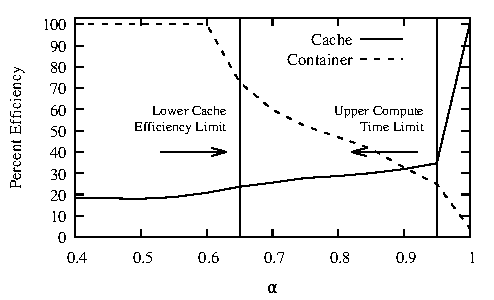
\includegraphics[width=0.9\linewidth]{curated/comparative/distribution_efficiency.pdf}

\parbox{\linewidth}{
Choosing $\alpha$ too low results in very poor cache efficiency (left line).
At high $\alpha$, the computational cost to prepare images becomes too high (right line).
The priorities of the particular application and site determine the ideal choice of $\alpha$.
Thus users or system administrators can balance storage, computational, and bandwidth costs to  significantly improve storage utilization.
}
\end{BlueBlock}

\end{minipage}
\end{frame}
\end{document}
